\documentclass{article}
\usepackage{graphicx} % Required for inserting images
\usepackage[utf8]{inputenc}
\usepackage[english]{babel}
\usepackage[tablegrid,nochapter]{vhistory} %%Vhistory simplifies the creation of a history of versions of a document
\usepackage[nottoc]{tocbibind} %%Automatically adds the bibliography and/or the index and/or the contents, etc., to the Table of Contents listing
\usepackage{authblk}
\usepackage{float}
\usepackage{longtable}
\usepackage[raggedrightboxes]{ragged2e}
\usepackage{titlesec}

\setcounter{secnumdepth}{4}
\setcounter{tocdepth}{4}

\titleformat{\paragraph}
{\normalfont\normalsize\bfseries}{\theparagraph}{1em}{}
\titlespacing*{\paragraph}
{0pt}{3.25ex plus 1ex minus .2ex}{1.5ex plus .2ex}

% Margins
\topmargin=-0.45in
\evensidemargin=0in
\oddsidemargin=0in
\textwidth=6.5in
\textheight=9.0in
\headsep=0.25in

\counterwithin{table}{subsection}

\def\BoldTitle{Követelményelemzés}
\def\Subtitle{Élő LEGO Projekt Irányításához\\}

\title{\textbf{\BoldTitle}\\\Subtitle}

\author{\textsc{\Large Projektvezető: Németh Gábor Árpád} \\ \textsc{Csapat tagjai:} Habzda Fruzsina Mária Horváth Sára, Kemény Dániel, Kiss Ámon, Novák Lilla, Racskó Balázs, Székely Szilárd, Torvinen Aili, Tóth Dóra, Vágó Blanka}

\date{\today}

\begin{document}

\maketitle

\pagebreak
\tableofcontents % Inhaltsverzeichnis

\pagebreak
\section{Revision History}

\begin{versionhistory}
    \vhEntry{1.0}{2023. November 3.}{Habzda Fruzsina Mária}{Első vázlat}
    \vhEntry{1.1}{2023. November 23.}{Novák Lilla}{A vázlat kibővítése és részekre osztása}
    \vhEntry{1.2}{2023. November 30.}{Tóth Dóra, Székely Szilárd}{Asztali, gyerekeknek szánt alkalmazás követelményei és felületterv megadása}
    \vhEntry{1.3}{2023. November 30.}{Horváth Sára, Novák Lilla}{Telefonos távirányító alkalmazás követelményei és felülettervek megadása}
    \vhEntry{1.4}{2023. December  1.}{Racskó Balázs, Vágó Blanka}{Fizikai távirányító követelményei és felületterv megadása}
    \vhEntry{1.5}{2023. December  3.}{Habzda Fruzsina}{Bevezető első verzió}
\end{versionhistory}


\pagebreak
\section{Projekt bemutatása}

Ennek a projektnek az lenne a célja, hogy LEGO-hoz hasonló elemek és robotok kompatibilitásával rendelkező távirányítót és programozási rendszert hozzunk létre. A távirányítás két részből áll: az applikációból és a fizikai távirányítóból. A programozáshoz két felület áll rendelkezésre. Továbbá tartozik egy megosztó fórum és felhasználói dokumentáció is a projekthez.
\newline

A célközönség minden korosztályt magába foglalja, a fő piac viszont egyelőre az Európai Unióra korlátozódik.
\newline

A programozási felület tartalmaz C++ fejlesztői környezetet és főként gyerekeknek szánt grafikus nyelvekhez felületet. Ez egy webalkalmazás formájában készül el, és a legelterjedtebb böngészőkben lesz támogatott. Az alkalmazás elemei, funkcionalitásai részletesen testreszabhatók, konfigurálhatók lesznek a hatékony felhasználás/használat érdekében. A grafikus felület színes formákkal segíti majd a programozást, és növeli az élményt a gyerekek számára. Az alkalmazásnak meg kell tudnia jeleníteni a vizuális programokat C++ nyelven is, hogy segítse a felhasználókat a bonyolultabb, csupán szöveges kódoláshoz való áttérésben.
A programok újrafelhasználhatók, megoszthatók egy fórumon, ahol értékelhetők is.
\newline

A fizikai távirányító elemekkel működik, Bluetooth-on keresztül kommunikál a robotokkal és a vezérlőegységekkel. Ez korlátozza a hatótávot. A fizikai távirányító főként a 8 éves korosztályt célozná meg. A távirányító funkciógombokat, analóg szabályzókat, LCD kijelzőt, Cím és Shift gombokat,  és on-off kapcsolót tartalmaz. EUs szabványnak meg kell felelnie, és ABS műanyagból kell készülnie.
\newline

A mobilapp távirányító Androidra, majd IOS-re támogatott ingyenes szoftver, és ez is Bluetooth-al kommunikál. A felhasználó testreszabhatja az applikációs felületet, mentheti és előhívhatja a beállításokat. A mobilapp elérhető nyelvei közé tartozik az angol, és az EU összes nyelve. Az alkalmazás tudja irányítani vezérlőegységhez csatlakoztatott perifériákat. (Ilyen perifériák lehetnek a kijelzők, motorok, lámpák, hangszórók és különböző érzékelők.)
\newline

A felhasználói dokumentáció az asztali alkalmazásról elérhető lesz az interneten. A C++ -os környezethez angol változat, a grafikus környezethez az EU összes nyelvén.
\newline

A projekt kivitelezése során fontos a perifériákat előállító csapattal való együttműködés.
\newline

A projekt időtartamára a megrendelővel nem történt megállapodás. 
Az általunk megbecsült költségvetés 150 millió Legófillért tesz ki.
\newline

Az alkalmazások és a felhasználói dokumentációk lefordításához speciálisan erre szakosodott alvállakozók bevonását javasoljuk. 
\newline

A dokumentációban található felülettervek javaslatok, nem a megrendelőtől származnak.


\pagebreak
\section{Követelmények}

követelmények számozása és felépítése (hogyan épül fel egy azonosító; követelménycsoport-id)
a megvalósítás fázisai (fázisok felsorolása, rövid leírása, követelményeik, időtartama) 
XY1 követelmény csoport követelményei (követelmények táblázatos leírása, azonosító, leírás)
XY2 ... \\
\\
\textit{(csak egy ötlet)} \\
C++ Programozási Felület - P \\
Grafikus Szerkesztő - G \\
Fizikai Távirányító - T \\
Mobilalkalmazás Távirányító - A \\
Webes Megosztás - W \\
Dokumentációs Anyag - D \\

\subsection{Programozási felületek}

(valami bevezető szöveg az adott részhez)

\subsubsection{C++ programozási felület}

(itt is valami bevezető szöveg az adott részhez)

\begingroup
\centering
\begin{longtable}{|c|p{14cm}|}
\hline
\textbf{Azonosító} & \textbf{Leírás}        \\ 
\hline
       \textbf{P\_00}  & … \\\hline
       \textbf{P\_00}  & … \\\hline
       \textbf{P\_00}  & … \\\hline
\hline
\caption{C++ programozási felület követelményei}
\end{longtable}
\endgroup


\subsubsection{Grafikus programozási felület}

A fiatalabb korosztályt megcélzó alkalmazás felülete 5 fő részből fog állni, amelyek segítségével a felhasználók könnyen és hatékonyan dolgozhatnak:

\begin{itemize}
\item \textbf{Navigációs sáv:} 
Az oldal tetején elhelyezkedő menü segítséget nyújt a fájlok kezeléséhez, beleértve a mentést, betöltést és egyéb fájlalapú műveleteket, amelyek segítségével könnyedén lehet tárolni és visszatölteni a kész programokat.
\item \textbf{Munkaterület:}
A Munkaterület a fő területe a felületnek, ahol a felhasználók programjaikat építhetik, szerkeszthetik és megtekinthetik. Ide helyezhetik el a különböző programozási elemeket az eszköztárból, melyeket könnyedén lehet mozgatni, valamint összekapcsolni egymással.
\item \textbf{Beállítások:} 
A jobb oldalon elhelyezkedő panel lehetőséget nyújt az elemek részletes beállításaira. Itt állíthatók az elemek specifikus tulajdonságai és paraméterei, ami további testreszabást és funkcionalitást biztosít a programoknak.
\item \textbf{Eszköztár:}
A bal oldalon található panelon számos programozási elem, mint például ciklusok, elágazások, hangvezérlő modulok és vizuális elemek állnak rendelkezésre. Ezek az eszközök könnyen hozzáférhetőek és húzhatók a fő felületre a program építése során.
\item \textbf{Programkód megjelenítő:}
Az oldal alján, a Programkód megjelenítőben a felhasználók által összeállított programok jelennek meg C++ formátumban. Ez az ablak segít a felhasználóknak megérteni a programozás logikáját és struktúráját, miközben átlépnek a vizuális programozásról a kódolás gyakorlatába.
\end{itemize}

\begin{figure}[H]
\centering
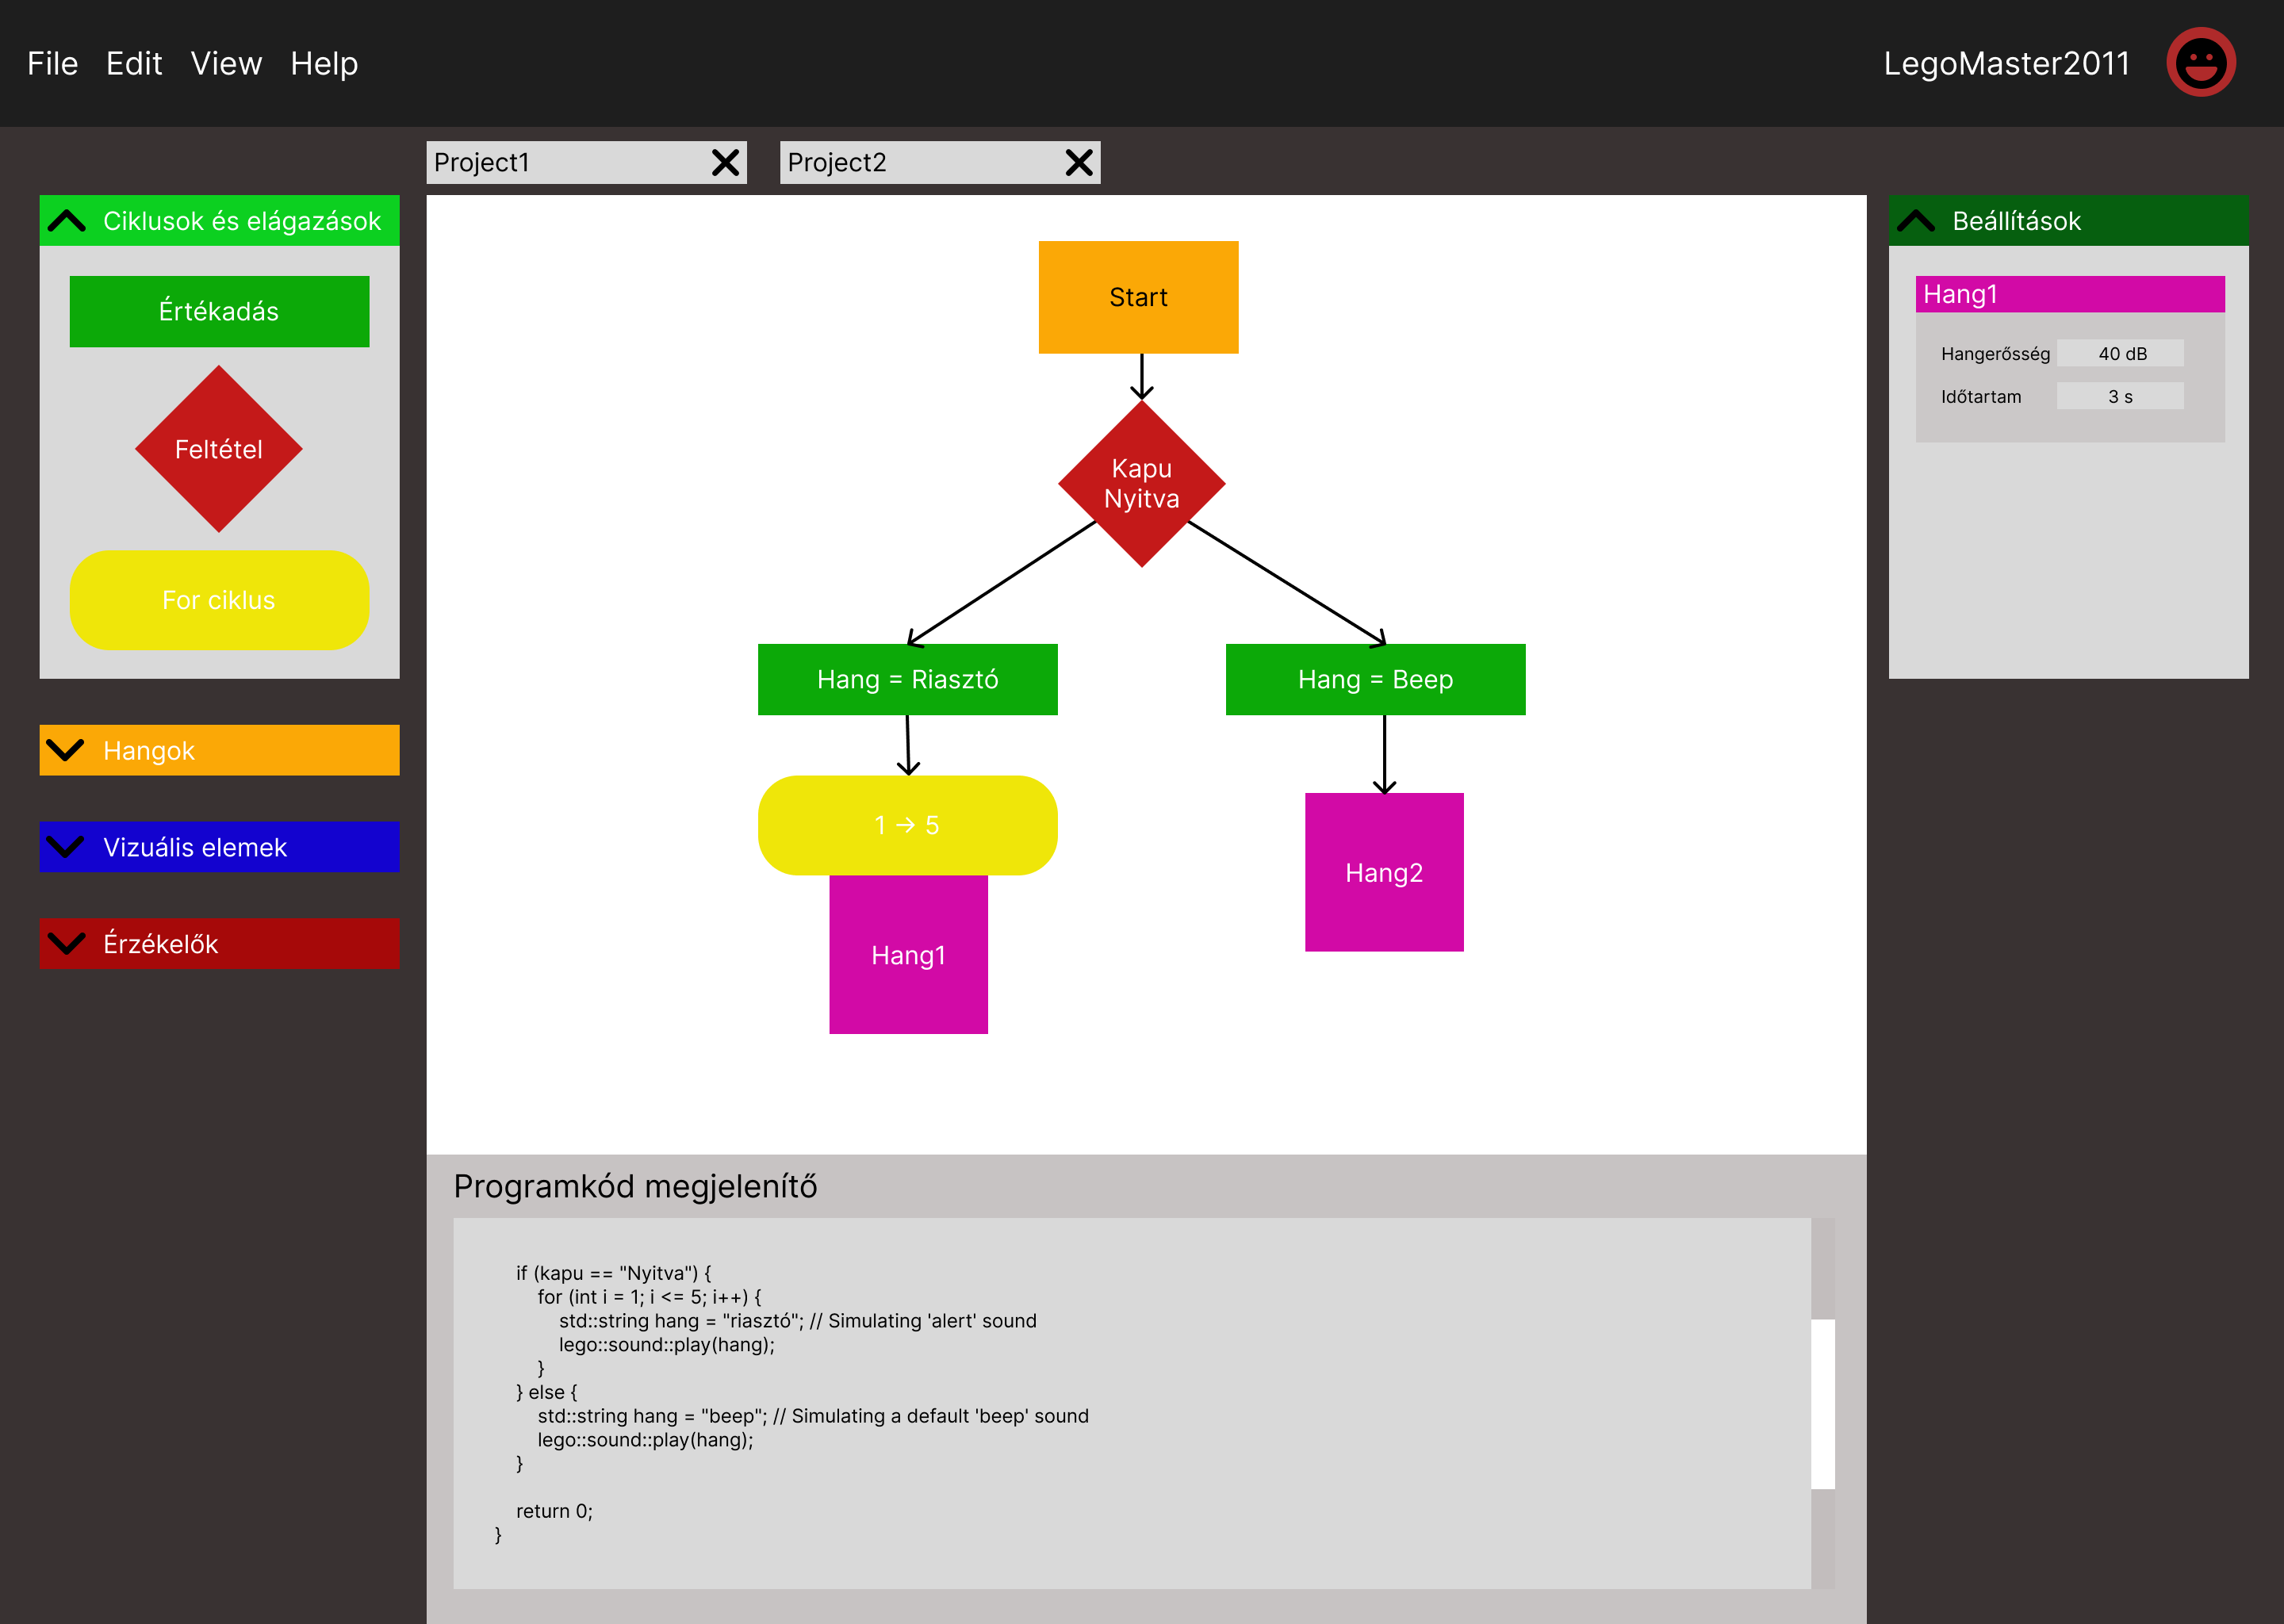
\includegraphics[width=1\linewidth]{gyerekeknek-felulet.png}
\caption{\label{fig:image}Gyerekeknek felület}
\end{figure}

\begingroup
\centering
\begin{longtable}{|c|p{14cm}|}
\hline
\textbf{Azonosító} & \textbf{Leírás}        \\ 
\hline
\textbf{G\_01} & Az alkalmazásnak lehetőséget kell biztosítania a lokális fájlok tárolására a vezérlőegységen belül, korlátozva a maximális 1GB tárhelyigényt. Későbbi fejlesztések során az alkalmazásnak támogatnia kell a fájlok megosztási lehetőségeit és a felhőalapú tárolást a további bővíthetőség érdekében \\\hline
\textbf{G\_02} & Az alkalmazásnak lehetőséget kell biztosítania a felhasználók számára a programjaik megosztására egy beépített fórum felületen keresztül. Ezen a fórumon a felhasználók megoszthatják saját kódjaikat, segítséget kérhetnek vagy értékeléseket adhatnak mások programjaira, lehetővé téve a közösségi tapasztalatok és segítségnyújtás megosztását a felhasználók között. \\\hline
\textbf{G\_03} & A programozói felületnek böngésző alapúnak kell lennie, támogatva a legelterjedtebb böngészőket: Chrome, Firefox, Safari, valamint Edge-t. Ennek révén biztosítva van a kompatibilitás és az optimális működés a felhasználók széles körű böngészőválasztéka esetén.\\\hline
\textbf{G\_04} & Az oldal tetején elhelyezkedő menürendszernek biztosítania kell a fájlok kezelését és egyéb fájlalapú műveleteket. Ennek részeként tartalmaznia kell olyan menüpontokat, mint a "File", "Edit", "View", "Help", valamint a jobb sarokban a felhasználó felhasználóneve. Ezek a menüpontok segítséget nyújtanak a fájlok mentéséhez, betöltéséhez és egyéb fájlalapú műveletek elvégzéséhez. \\\hline
\textbf{G\_05} & A jobb oldalon elhelyezkedő panel funkciójának ki kell terjednie az elemek részletes beállításaira. Ezen a felületen a felhasználóknak lehetőséget kell biztosítani arra, hogy az egyes elemek specifikus tulajdonságait és paramétereit testre szabhassák. Ennek révén a felhasználóknak képesnek kell lenniük részletesen finomhangolni az elemek működését és megjelenését, továbbá lehetőséget kell adni a funkcionalitás bővítésére a programokban. Az elemek részletes konfigurálhatósága növeli a rugalmasságot és segíti a felhasználókat az alkalmazásban való hatékonyabb és testreszabottabb munkavégzésben. \\\hline
\textbf{G\_06} & A bal oldalon található panelen elérhetőnek kell lennie a következő programozási elemeknek:
\begin{itemize}
    \item Ciklusok és elágazások
    \item Hangvezérlő modulok
    \item Vizuális elemek
    \item Érzékelők
\end{itemize}

Ezeknek az eszközöknek könnyen hozzáférhetőnek és használhatónak kell lenniük, ezért egy lenyíló listában kell elhelyezkedniük, lehetővé téve a felhasználók számára azok egyszerű húzását és elhelyezését a fő felületre a programok építése során.\\\hline

\textbf{G\_07} & A vizuális elemek alakzatok formájában jelennek meg és különböző színekkel rendelkeznek, hogy a gyerekek számára könnyen használható legyen. \\\hline
\textbf{G\_08} & Az oldal alján található Programkód megjelenítő felületen kell megjeleníteni a felhasználók által összeállított programokat C++ formátumban. Ez az ablak fontos szerepet tölt be azzal, hogy segítse a felhasználókat a programozás logikájának és struktúrájának megértésében, miközben átmennek a vizuális programozásból a kódolás gyakorlatába. A megjelenítő felületnek pontosan és érthetően kell bemutatnia a kódokat, hogy a felhasználók könnyen olvashassák, megérthessék és tanulhassanak belőlük a kódolási folyamat során.\\\hline

\textbf{G\_09} & A Munkaterületnek a fő részének kell lennie az alkalmazáson belül, ahol a felhasználók a programjaikat létrehozhatják, szerkeszthetik és megtekinthetik. Ide kell helyezni és rendezni a különböző programozási elemeket az eszköztárból, hogy a felhasználók könnyedén elhelyezhessék és mozgathassák azokat a Munkaterületen.\\\hline

\textbf{G\_10} & Az elemek közötti mozgatásnak és kapcsolatok kialakítása nyilak segítségével valósítandó meg, hogy egyszerű és intuitív legyen, hogy a felhasználók gördülékenyen és hatékonyan tudjanak dolgozni a programjaik létrehozásakor. \\\hline
\hline
\caption{Gyerekeknek szánt felület követelményei}
\end{longtable}
\endgroup

\subsection{Távirányítók}
\subsubsection{Fizikai Távirányítás}
\subsubsection{Felület terv}

\begin{figure}[H]
\centering
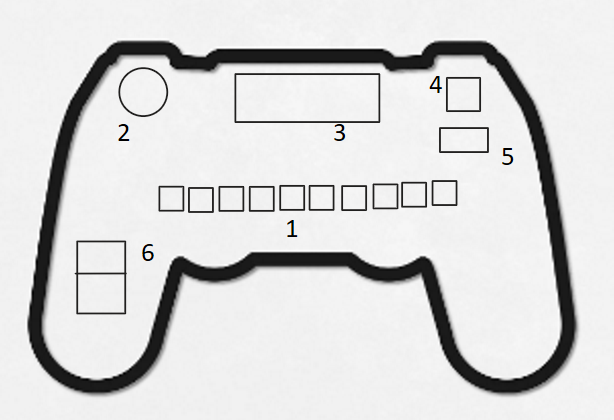
\includegraphics[width=1\linewidth]{fizikaitavir_feluletter.png}
\caption{\label{fig:image}Fizikai távirányító}
\end{figure}


\paragraph{Funkciók}

\begingroup
\centering
\begin{longtable}{|c|p{14cm}|}
\hline
\textbf{Azonosító} & \textbf{Leírás}        \\ 
\hline
       \textbf{T\_01}  & Funkciógombok
       \begin{itemize}
        \item Előre meghatározott funkciókat indítanak el, amennyiben az adott funkciót támogatja a jelenleg kapcsolódott vezérlő egység.
        \item Tíz darab, 0-9-ig számozva.
        \item Megnyomásra a kijelzőn az aktuálisan kiválasztott vezérlőegység kódja mellett megjelenik a funkció sorszáma is.
        \end{itemize}
       \\\hline
       \textbf{T\_02}  & Analóg Szabályzó 
       \begin{itemize}
        \item Folytonos állású körbetekerhető kapcsoló.
        \item Funkciótól függően különböző dolgokat szabályoz. (Pl.: sebesség, fényerő stb)
        \item Tekerés közben 3 másodpercig a kijelzőn megjelenik a jelenleg választott érték, az adott funkció értéktartományától függően.
        \item 1 teljes körbetekerés 100 egység.
        \end{itemize}
       \\\hline
       \textbf{T\_03}  & LCD Kijelző
       \begin{itemize}
        \item Minden információ itt jelenik meg.
        \item Alapesetben a kiválsaztott vezérlő 7 jegyű kódja és a funkció sorszáma van kijelezve. 
        \item Alacsony akkufeszültség esetén “LOW BATT” jelzést mutat, felváltva villog az alap kiválasztással.
        \item Kiválasztott vezérlő nélkül “NO SIGN” jelzés látható.
        \end{itemize}
       \\\hline
       \textbf{T\_04}  & Cím Gomb 
       \begin{itemize}
        \item Aktuálisan vezérelt egységek közötti váltógomb
        \end{itemize}
       \\\hline
       \textbf{T\_05}  & Shift Gomb 
       \begin{itemize}
        \item További funkciók elérése 10-19ig a megfelelő funkciógomb megnyomásával. 
        \end{itemize}
       \\\hline
       \textbf{T\_06}  & On-Off Kapcsoló 
       \begin{itemize}
        \item Kétállású váltókapcsoló
        \item A távirányító ki-be kapcsolására alkalmas gomb.
        \item Kikapcsoláskor a Bluetooth kapcsolat is megszakad, így a jelenleg futó funkció leáll
        \item Bekapcsoláskor alapértelmezésben nem kapcsolódik vezérlőegységhez, 0-s funkció kerül kiválasztásra.
        \end{itemize}
       \\\hline
       
\hline
\caption{Fizikai távirányító követelményei}
\end{longtable}
\endgroup

\paragraph{Anyaghasználat}
    \begin{itemize}
        \item 100\% ABS Műanyag
    \end{itemize}


\paragraph{Kapcsolódási specifikáció}
\begin{itemize}
    \item Bluetooth 2.0 szabvány szerint
    \item 100m hatótávolság
    \item Ezen a kapcsolódási módon keresztül lehetőség a távirányító firmwarejének frissítésére, applikáción keresztül.
\end{itemize}

\paragraph{Energiaellátás}
\begin{itemize}
    \item AAA elem (vagy akkumulátor), 2db (Nem tartozék)
    \item Működési feszültség 3V
\end{itemize}

\paragraph{Biztonsági tudnivalók}
\begin{itemize}
    \item EU Szabványnak megfelelő termék
    \item 8+ (Nyolc éves kortól használható)
\end{itemize}


\subsubsection{Telefonon és tableten elérhető applikáció követelményei}

Az tervezett alkalmazás mobil és táblagép platformokon elérhető lesz. Az fejlesztés két fázisra oszlik: az Android verzió az első fázisban jelenik meg, majd a másodikban következik az iOS változat. Mindkét verzió ingyenes lesz és támogatni fogja a legfrissebb operációs rendszereket. Az alkalmazás lehetővé teszi távirányítók létrehozását, testreszabását és irányítást Bluetooth kapcsolaton keresztül. A felhasználók képesek lesznek kijelzőket, LED lámpákat, motorokat, hangszórókat és érzékelőket irányítani az alkalmazás segítségével, valamint létrehozhatnak és kezelhetnek különböző távirányító felületeket.

\paragraph{Követelmények}
\begingroup
\centering
\begin{longtable}{|c|p{14cm}|}
\hline
\textbf{Azonosító} & \textbf{Leírás}        \\ 
\hline
       \textbf{A\_01}  & Az alkalmazás elérhető lesz mobilon és táblagépen egyaránt. A fejlesztés két fázisra oszlik: az Android alkalmazás az első fázisban készül el, míg a második fázisban az iOS alkalmazás fejlesztése történik. Az Android alkalmazás kompatibilis lesz az Android 11. verziótól kezdve, és támogatni fogja az újabb Android verziókat is (pl. Android 12, 13 stb.). Az iOS alkalmazás elérhető lesz az iOS 14 verziótól kezdve és támogatja az ezt követő újabb iOS verziókat. Az Android alkalmazás elérhető lesz a Google Play Áruházban. Az iOS alkalmazás elérhető lesz az App Store-ban. Az alkalmazás mindkét platformon ingyenesen elérhető a felhasználók számára. Az alkalmazás támogatja a sötét módot, amely összhangban van a felhasználó által beállított telefon vagy táblagép rendszereinek sötét mód beállításaival. \\\hline
       
       \textbf{A\_02}  & Az alkalmazás menürendszerében a következő opcióknek kell megjelennie:
       \begin{itemize}
       \item "Console"
       \item "Templates"
       \item "Editor"
       \item "Settings"
       \end{itemize}
       A “Console” menüpontban érhető el az aktuális távirányító. A “Templates” menüben láthatja a felhasználó az összes korábban mentett távirányítót, lehetőség van egy távirányíttót aktuális távirányítóvá választani és kedvencekként megjelölni ezeket. Az “Editor” menüpontban készíthet a felhasználó új távirányítókat és  szerkeszthet már meglévőket. A “Settings” menüpontban az alkalmazás nyelvének módosítása lehetséges. \\\hline
       
       \textbf{A\_03}  & Az alkalmazás felhasználói felülete elérhető lesz az Európai Unió (EU) nyelvein. A felhasználóknak lehetőségük lesz könnyen átállítani az alkalmazás nyelvbeállításait az alkalmazás "Beállítások" menüjében. Az alkalmazáshoz készül egy felhasználói dokumentáció, amely egy külső weboldalon lesz elérhető. A dokumentáció minden EU nyelvén elérhető lesz, hogy segítse a felhasználókat az alkalmazás megértésében és kezelésében.  \\\hline
       
       \textbf{A\_04}  & Az alkalmazás alapértelmezett felületi tervvel rendelkezik, amely tartalmazza az összes funkciógombot és optimalizált elrendezést kínál. Az alkalmazás alapfelülete részben hasonlítani fog a hagyományos fizikai távirányítók elrendezésére és funkcióira. Emellett a felhasználóknak lehetőségük van saját felület és kinézet tervezésére a távirányítóhoz. A felhasználók testreszabhatják és alakíthatják az alkalmazás távirányító felületét a saját igényeiknek és LEGO modelljeiknek megfelelően. Az alkalmazás lehetőséget biztosít a felhasználóknak arra, hogy a távirányító kialakításához előre meghatározott funkció gombokat húzzanak és helyezzenek el az alkalmazásban a drag-and-drop módszer segítségével. A funkciógombok számának, elrendezésének és elhelyezkedésének meghatározására is lehetőség nyílik. Ezen felül a felhasználók meghatározhatják, hogy melyik vezérlőegység melyik portjához rendelik ezeket a funkciógombokat, így lehetővé téve a kiválasztott perifériák vezérlését az alkalmazáson keresztül. \\\hline
       
       \textbf{A\_05}  & Az alkalmazás lehetőséget biztosít több különböző felület létrehozására. A felhasználók által létrehozott távirányítókat nevekkel ellátva lehet menteni. A felhasználóknak lehetőségük van új felületeket létrehozására, vagy korábban mentett felületek módosítására az igényeiknek megfelelően. Exportálni és importálni is lehet a mentett felületeket. Az exportált és importált távirányító felületek fájlformátuma JSON. Az alkalmazásban a felhasználóknak lehetőségük van új távirányítókat létrehozni üres felülettel, vagy már meglévőket módosítani a "Szerkesztés" gomb segítségével. Azonban a háttérkép vagy más megjelenési elemek nem módosíthatóak vagy személyre szabhatóak a felhasználók által. \\\hline
       
       \textbf{A\_06}  & A szerkesztési felületen elérhető lesz egy funkciógomb készlet, amely gombokat, kapcsolókat, csúszkákat, tekerőket és kijelzőket foglal magában. Ezen a felületen a felhasználók képesek lesznek kiválasztani és beilleszteni az egyes funkciógombokat a távirányító felületére. A felület szerkesztése során az alkalmazásban található gombok inaktív állapotban vannak. Ennek célja, hogy a felhasználók könnyedén elhelyezhessék és testre szabhassák a felületet anélkül, hogy véletlenül aktiválnák a gombokat a szerkesztés folyamán. Az alkalmazásban a felhasználó elnevezheti a funkciógombokat, ahol a név maximum 8 alfanumerikus karakter hosszúságú lehet. A funkciógomb neve a gomb felett fog megjelenni. Emellett lehetőség van a gombok címzésének módosítására is, ami alapértelmezetten az 1-es vezérlőegység 1-es portjára mutat a funkciógomb kihelyezése után. Ezt az alap beállítást bármikor megváltoztathatja a felhasználó igényei szerint. Amikor a távirányító tervezése befejeződik, a "Mentés" gombbal tudja elmenteni az elkészült konfigurációt. \\\hline

       \textbf{A\_07}  & Az alkalmazás Bluetooth kapcsolaton keresztül irányítja a vezérlőegységeket, és a távirányítónak a Bluetooth 2.0 specifikáció által meghatározott távolságig kell működnie. Az alkalmazás és a fizikai távirányító közötti adatcsere nem szükséges. Az alkalmazást párosítani kell a vezérlőegységgel, hogy az aalkalmazás képes legyen irányítani az adott vezérlőegységet. Amikor össze akarjuk párosítani a fizikai távirányítót az alkalmazással és a vezérlőegységgel, az a vezérlő fogja irányítani a vezérlőegységet, amellyel utoljára párosítva volt. Az alkalmazás és a fizikai távirányító ebben az összefüggésben egyenrangúak, és az utoljára létrejött párosítás határozza meg, hogy melyik irányítja a vezérlőegységet. \\\hline
       
       \textbf{A\_08}  & - Az alkalmazás képes irányítani a következő vezérlőegységekre csatlakoztatott perifériákat:
       \begin{itemize}
       \item Motor
       \item Pixeles kijelző
       \item LED lámpa
       \item Hangszóró
       \item Érzékelők
         \begin{itemize}
         \item Reed relé
         \item Nyomógomb
         \item Kétállású ki-be kapcsoló
         \item Távolság-, fényerő- és szín érzékelő
         \item Giroszkóp
         \end{itemize}
       \end{itemize} \\\hline

       \textbf{A\_09}  & Az alkalmazás funkciógomb készletében számos gomb található. A motor fordulatszámát a felhasználó állíthatja 0-tól 20-ig, ezzel meghatározva a sebességet. Emellett a motor képes visszajelzést adni a pozíciójáról és a fordulatszámáról, amit a kijelzőn meg tud jeleníteni a felhasználó. A felhasználó grafikát jeleníthet meg a pixeles kijelzőn. A kijelzők pixelei képesek RGB színeket megjeleníteni, és a felhasználónak lehetősége van több különálló kijelzőt egyenként kezelni. Alapértelmezés szerint ez az opció be van kapcsolva, de a felhasználó kikapcsolhatja, ha szükséges. A kijelzőn megjelenített grafikát a vezérlőegység határozza meg, ezért a felhasználónak először feltöltetnie kell a kívánt grafikát a vezérlőegységre. A LED állapotát a vezérlőegység vezérli, a felhasználó pedig a színkerék segítségével kiválaszthatja a színt, vagy manuálisan adhatja meg a HEX kódot. A felhasználó képes irányítani a hangszórót, választhat alap hangok közül vagy saját hangokat tölthet fel a vezérlőegységre. Az adott hang lejátszását egy legördülő menüből választhatja ki, majd a "Lejátszás" gombbal indíthatja el. A kijelző jelzi a vezérlőegység által végrehajtott utasításokat az adott porton, és visszajelzi, hogy azok sikeresek vagy sikertelenek voltak. Továbbá a kijelző képes megjeleníteni más érzékelők visszajelzéseit, mint például a reed relé, nyomógomb, kétállású ki-be kapcsoló, távolság-, fényerő- és színérzékelő, valamint a giroszkóp jelzéseit. A színérzékelés esetén nemcsak a HEX kód, hanem maga a szín is megjelenik a kijelzőn. A címzőgombok lehetővé teszik a felhasználó számára, hogy az egyes funkciógombokat hozzárendelje egy vezérlőegység portjához. A gombok felett megjelenik a vezérlőegység sorszáma vagy neve (ha van), valamint a port sorszáma. Ez lehetővé teszi, hogy a felhasználó több ugyanolyan funkciógombot helyezzen el a felületen, amelyek különböző perifériákat irányítanak. \\\hline
       
\hline
\caption{Telefonos és tabletes távirányító követelményei}
\end{longtable}
\endgroup

\paragraph{Felületi tervek}

\begin{figure}[H]
\centering
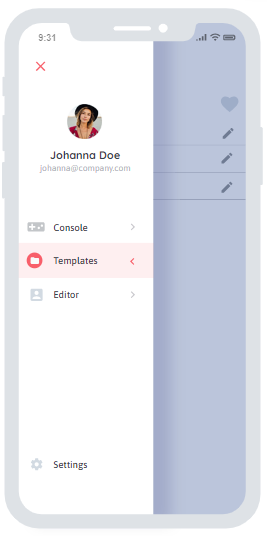
\includegraphics[height=1\linewidth]{Menu.png}
\caption{\label{fig:image}Telefonos és tabletes távirányító menü felületi terve}
\end{figure}

\begin{figure}[H]
\centering
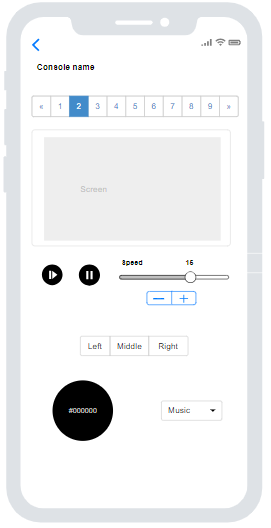
\includegraphics[height=1\linewidth]{console.png}
\caption{\label{fig:image}Telefonos és tabletes távirányító egyéni vezérlőpult felületi terve}
\end{figure}

\begin{figure}[H]
\centering
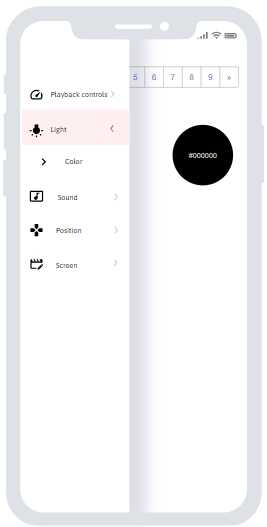
\includegraphics[height=1\linewidth]{vezerlopult_testreszabas.png}
\caption{\label{fig:image}Telefonos és tabletes távirányító egyéni vezérlőpult testreszabás felületi terve}
\end{figure}

\begin{figure}[H]
\centering
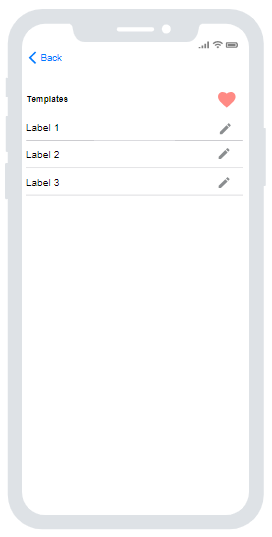
\includegraphics[height=1\linewidth]{egyeni_vezerlopultok.png}
\caption{\label{fig:image}Telefonos és tabletes távirányító egyéni vezérlőpult lista felületi terve}
\end{figure}

\subsection{Weboldal}
(rövid bevezető)

\subsubsection{Megosztási felület}
(rövid bevezető)

\begingroup
\centering
\begin{longtable}{|c|p{14cm}|}
\hline
\textbf{Azonosító} & \textbf{Leírás}        \\ 
\hline
       \textbf{M\_00}  & … \\\hline
       \textbf{M\_00}  & … \\\hline
       \textbf{M\_00}  & … \\\hline
\hline
\caption{…}
\end{longtable}
\endgroup


\subsubsection{Dokumentáció}
(rövid bevezető)

\begingroup
\centering
\begin{longtable}{|c|p{14cm}|}
\hline
\textbf{Azonosító} & \textbf{Leírás}        \\ 
\hline
       \textbf{D\_00}  & … \\\hline
       \textbf{D\_00}  & … \\\hline
       \textbf{D\_00}  & … \\\hline
\hline
\caption{…}
\end{longtable}
\endgroup


\pagebreak
\section{Szójegyzék}

(szavak csoportosítva, definíciókkal ellátva)

\end{document}
